\chapter{Text detection}
\label{chap:text-detection}


\section{Introduzione}
Negli ultimi anni, con l'avvento delle tecnologie di intelligenza artificiale e machine learning, gli algoritmi di rilevamento e riconoscimento del testo (\textit{text detection and recognition}) hanno subito un'evoluzione radicale, sia dal punto di vista dell'accuratezza dei risultati che dal punto di vista del tempo di esecuzione. Per quanto riguarda la \textit{text recognition} basta osservare il salto di qualit\`a subito da motori OCR open-source, quali \textit{Tesseract}, a seguito dell'implementazione di reti neurali ricorrenti (\textit{RNN}) di tipo \textit{LSTM} (\textit{Long Short Term Memory}), particolarmente adatte per questo tipo di applicazioni.\par
In questo capitolo ci concentriamo sull'introduzione di alcuni algoritmi di \textit{text detection}, che vengono utilizzati per riconoscere regioni di testo presenti in un'immagine e presentiamo un integrazione efficiente di questi metodi all'interno della libreria QI-OCR. 


\section{MSER}
Il metodo presentato in \cite{bib:mser} \`e un algoritmo di \textit{blob\footnote{Un blob in un'immagine \`e un gruppo connesso di pixel che condividono una determinata propriet\`a.} detection}, per la rilevazione di alcuni regioni distinguibili (\textit{DRs - Distinguished Regions}) in un'immagine, ovvero regioni che posseggono propriet\`a di stabilit\`a e invarianza, con un conseguente alto grado di ripetibilit\`a nella rilevazione.\par
Introduciamo delle regioni che vengono denominate \textit{ER (Extremal Regions)}, nel senso che tutti i pixel interni hanno intensit\`a esclusivamente maggiore o minore dei pixel nel contorno esterno della regione. Le \textit{ER} godono di due importanti propriet\`a: sono invarianti per trasformazioni geometriche affini e per trasformazioni monot\`one di intensit\`a dell'immagine. Le regioni di interesse sono un sottoinsieme delle \textit{ER} e vengono denominate \textit{MSER} (\textit{Maximally Stable Extremal Regions}), poich\`e risultano \textit{stabili} sotto una serie di operazioni di \textit{thresholding} e permettono una rilevazione multi-scala delle regioni, nel senso che vengono individuate sia strutture molto piccole che molto grandi.\par
Il grande vantaggio di questo \textit{blob detector} \`e la sua efficienza, in quanto l'enumerazione di tutte le \textit{ER} ha una complessit\`a temporale quasi lineare\footnote{In \cite{bib:mser-linear} \textit{Nist\'er} e \textit{Stew\'enius} propongono un metodo per l'enumerazione delle \textit{MSER} in tempo $\mathcal{O}(n)$, lineare nel numero di pixel dell'immagine.} di $\mathcal{O}(n\log{}\log{}n)$, data principalmente dall'algoritmo di enumerazione delle componenti connesse\footnote{Esiste una versione pi\`u efficiente, ma pi\`u articolata, dell'algoritmo per il \textit{labeling} delle componenti connesse (\textit{Rosenfeld-Pfaltz} \cite{bib:connected-components-fast}) con complessit\`a $\mathcal{O}(n\alpha(n))$, con $\alpha$ inversa della funzione di \textit{Ackermann}.}, con $n$ numero di pixel dell'immagine.\par
Nella pratica, l'algoritmo presentato pu\`o essere adattato per vari scopi e in particolare per il riconoscimento di testo in ambienti naturali, come descritto in \cite{bib:mser-canny}.\par
In figura \ref{fig:mser} un esempio di \textit{text detection} con l'utilizzo dell'algoritmo \textit{MSER} implementato nella libreria \textit{OpenCV}:
\begin{figure}[h]
	\centering
	\resizebox{\textwidth}{!}{
		\centering
		\subfloat[Input] {%
			\scalebox{0.5}[0.5] {
				\frame{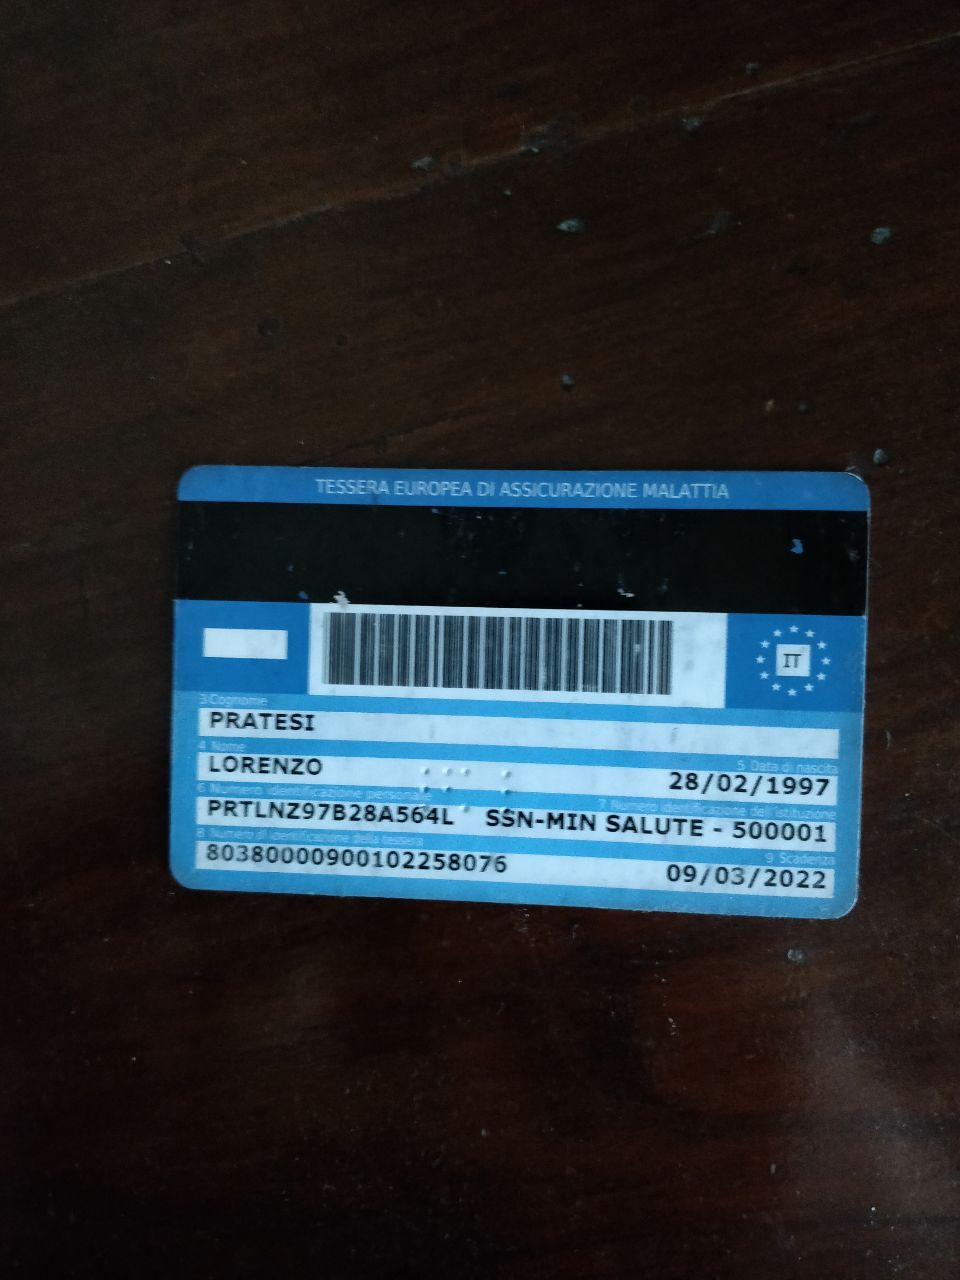
\includegraphics[width=.5\linewidth]{img/mser-east-input.png}}
			}
		}
		\subfloat[Output] {%
			\scalebox{0.5}[0.5] {
				\frame{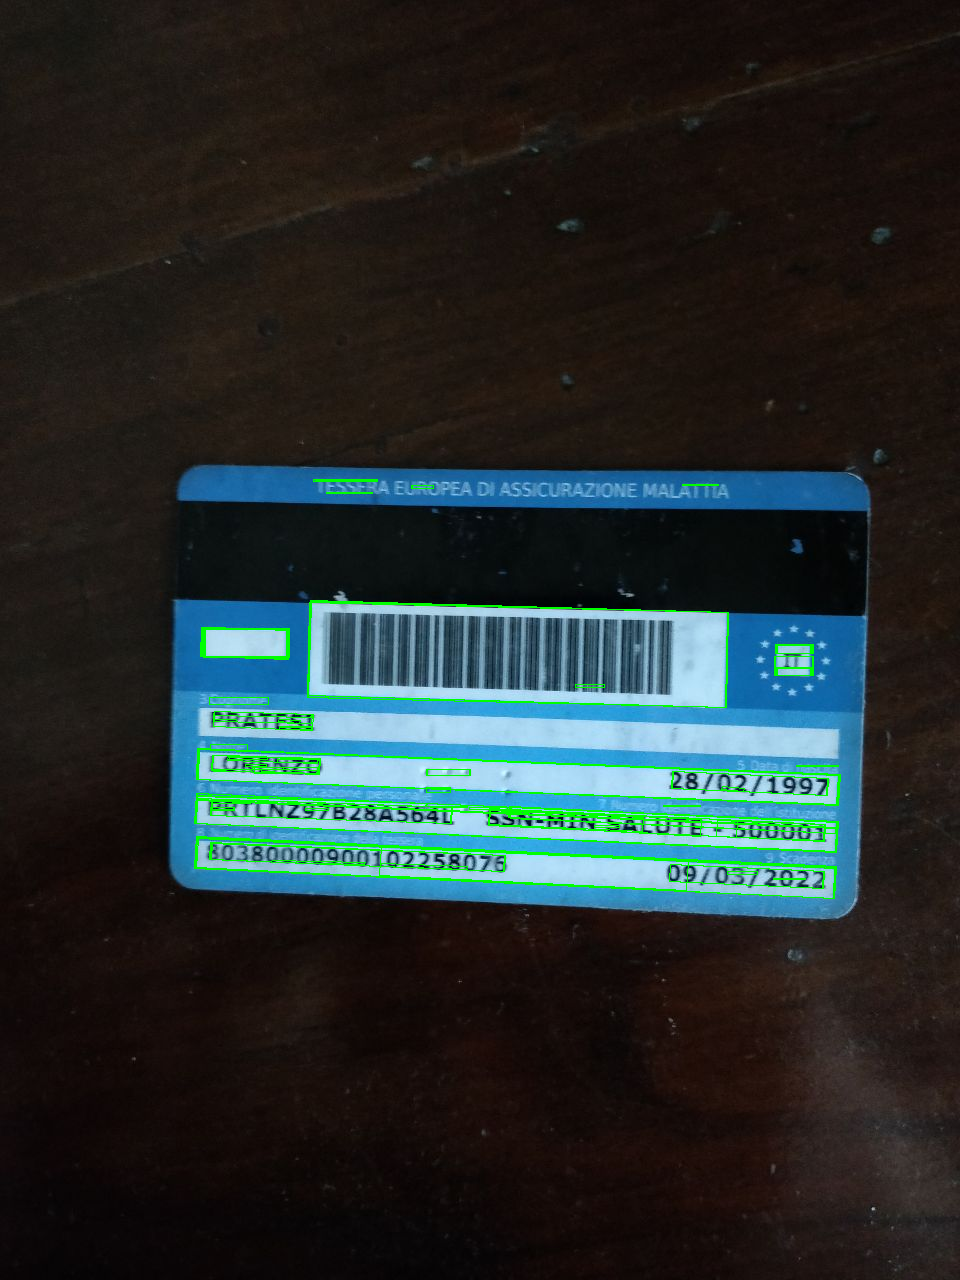
\includegraphics[width=.5\linewidth]{img/mser-regions.png}}
			}
		}
		\subfloat[][Output filtrato] {%
			\scalebox{0.5}[0.5] {
				\frame{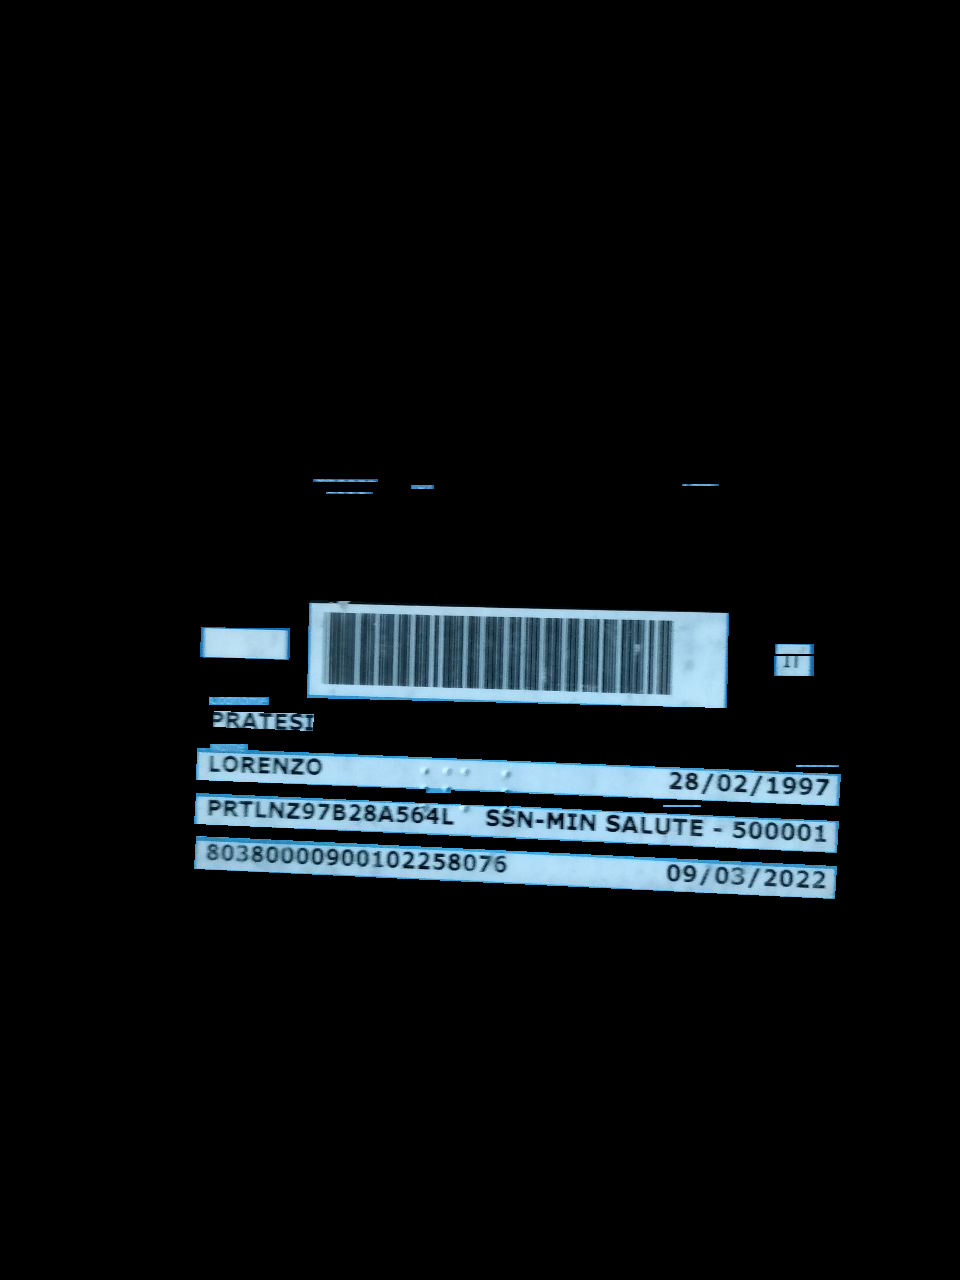
\includegraphics[width=.5\linewidth]{img/mser-regions-filtered.png}}
			}
		}
	}
	\caption{Text detection con \textit{MSER}} \label{fig:mser}
\end{figure}


\section{EAST}
L'approccio ideale per i problemi di \textit{text detection} sarebbe quello di utilizzare un algoritmo che prende in input un'immagine e restituisce una lista di rettangoli, in cui ciascun rettangolo identifica una regione di testo dell'immagine. In base al tipo di \textit{text detection} che si intende effettuare, non orientata o orientata, ciascun rettangolo \`e identificato, rispettivamente, da una coppia $(x, y)$, $lunghezza$ e $altezza$, oppure da 4 coppie $(x, y)$ per ciascun vertice del rettangolo. Osservando l'output prodotto da \textit{MSER} in figura \ref{fig:mser}, \`e possibile constatare che le regioni restituite non sono solamente quelle contenenti testo. Infatti, nell'esempio riportato, viene evidenziata anche la regione contenente il \textit{codice a barre} del documento.\par 
\textit{EAST} (\textit{Efficient and Accurate Scene Text detector}) \cite{bib:east} cerca di superare i limiti di \textit{blob detector} come \textit{MSER}, tramite l'implementazione di una rete neurale convoluzionale (\textit{FCN - Fully Convolutional Network}). Le specifiche di questa soluzione non rientrano negli obiettivi di questa tesi, ma nelle figure \ref{fig:mser} e \ref{fig:east} presentiamo un esempio di immagine processata sia da \textit{MSER} che dalla rete \textit{EAST}, per poter confrontare i risultati ottenuti.
\begin{figure}[h]
	\centering
	\resizebox{\textwidth}{!}{
		\centering
		\subfloat[Input] {%
			\scalebox{0.5}[0.5] {
				\frame{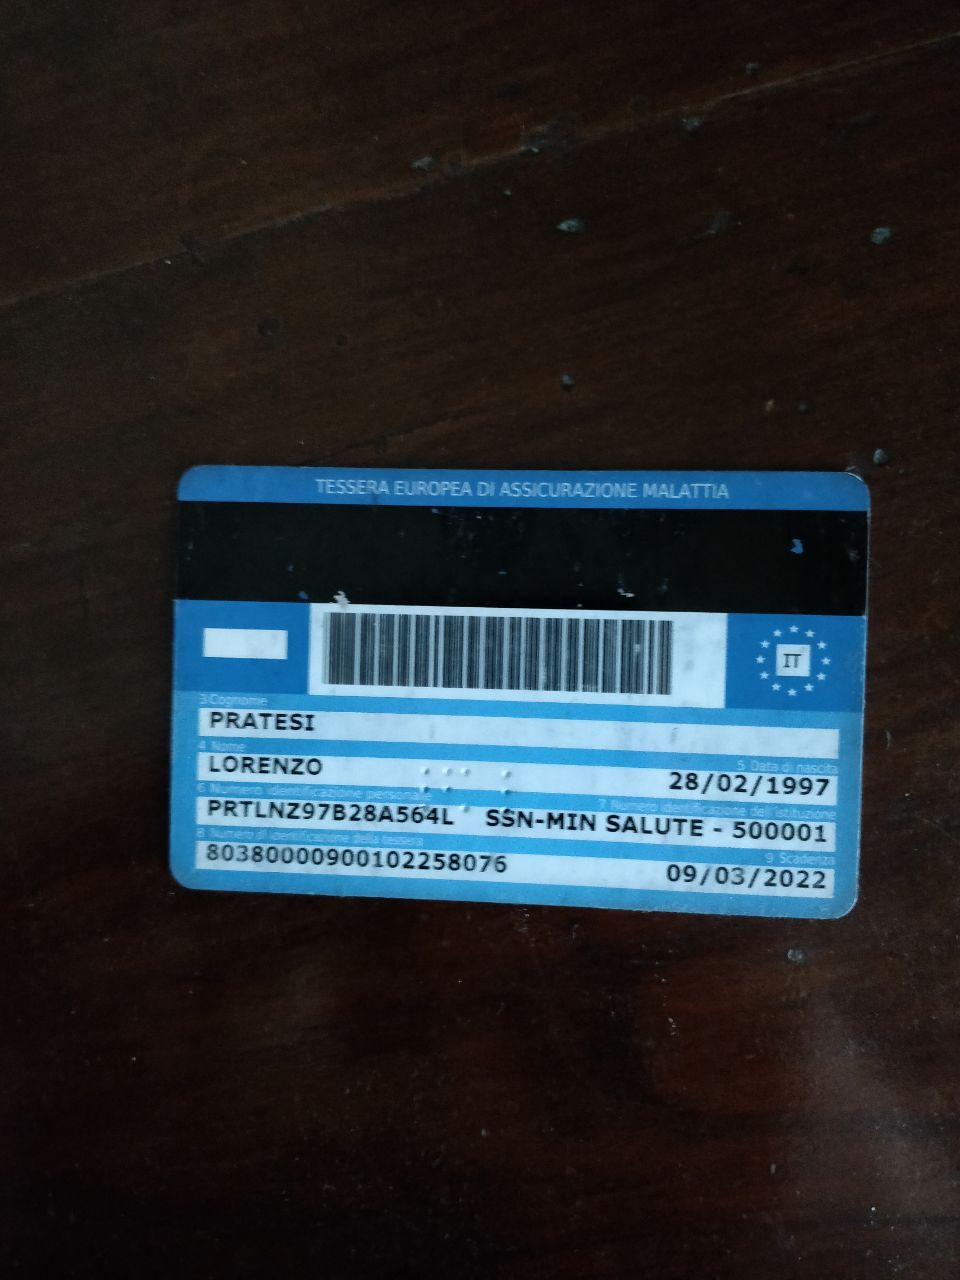
\includegraphics[width=.8\linewidth]{img/mser-east-input.png}}
			}
		}
		\subfloat[Output] {%
			\scalebox{0.5}[0.5] {
				\frame{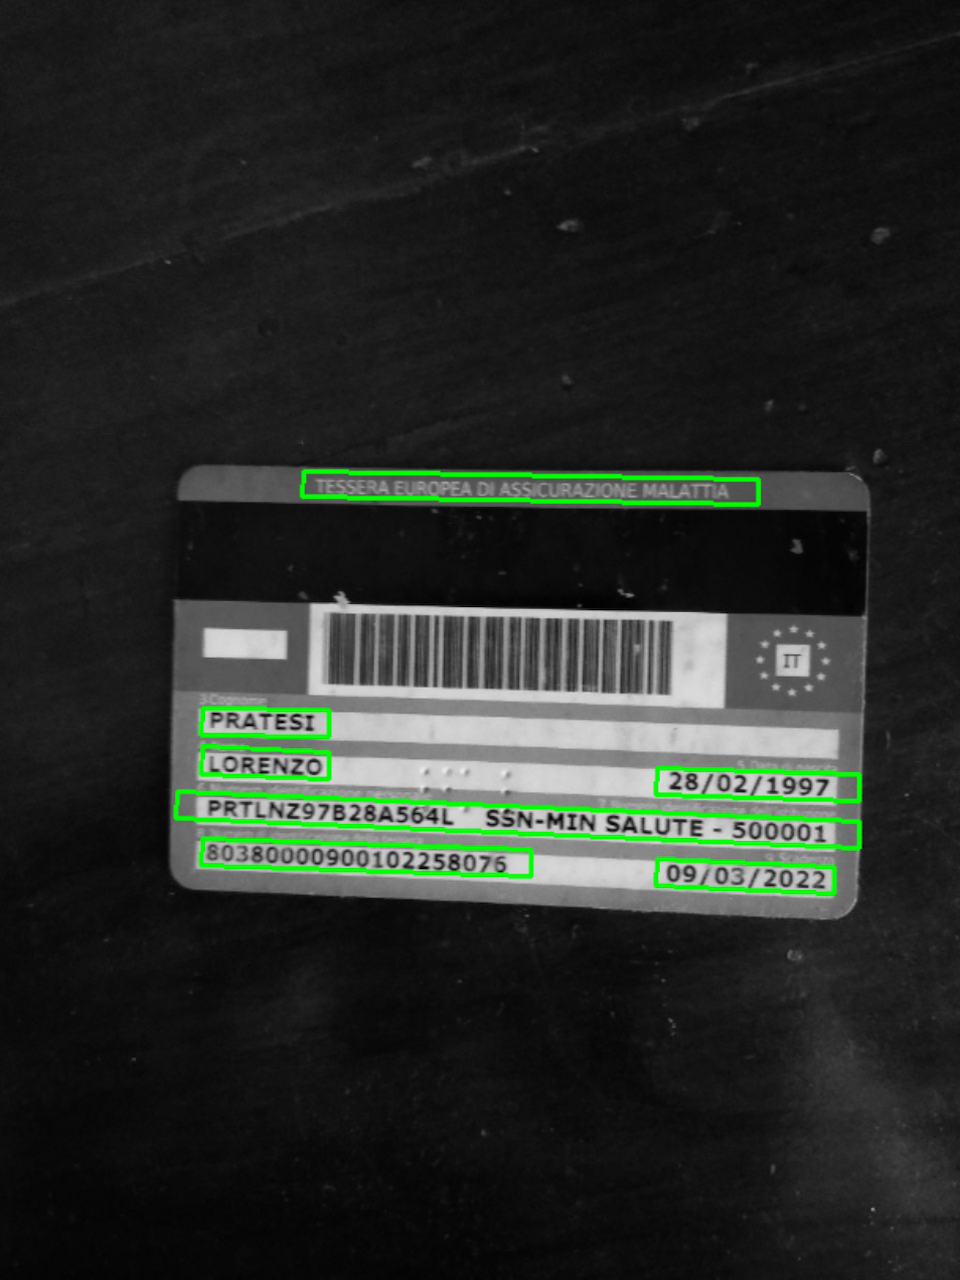
\includegraphics[width=.79\linewidth]{img/east-output.png}}
			}
		}
	}
	\caption{Text detection con \textit{EAST}} \label{fig:east}
\end{figure}


\section{Algoritmo proposto}
